\documentclass[12pt,a4paper]{article}
\usepackage[UTF8]{ctex}
\usepackage{amsmath,amssymb}
\usepackage{xcolor}
\usepackage{hyperref}
\usepackage{geometry}
\usepackage{graphicx}
\geometry{margin=2.5cm}

\title{Quantum Phase Estimation}
\author{QuoNic}
\date{}

\begin{document}
\maketitle

\begin{center}
\textbf{Algorithms} | Difficulty: Advanced | Time: 15 min
\end{center}

\tableofcontents
\newpage

\section{Why do we need it?}

Quantum Phase Estimation (QPE) is the core of many quantum algorithms, used to estimate eigenvalues of unitary operators.

\subsection{Classical Limitations}
\begin{itemize}
  \item Classical methods cannot efficiently estimate quantum state phases
  \item For large quantum systems, classical methods require exponential time
\end{itemize}

\subsection{Quantum Advantages}
\begin{itemize}
  \item QPE can efficiently estimate eigenvalues of unitary operators
  \item Core of Shor's algorithm, quantum chemistry simulation
  \item Provides exponential speedup
\end{itemize}

\subsection{Real-world Applications}
\begin{itemize}
  \item Shor's Algorithm (factoring)
  \item Quantum Chemistry (molecular energy calculation)
  \item Quantum Machine Learning (kernel methods)
\end{itemize}

\section{Quick Start}

\begin{verbatim}
from quonic import qgate, qshow
from quonic.gates import H, X

# Simple QPE example
qgate(X, 1)  # Prepare eigenstate
qgate(H, 0)  # Superposition
qgate(CU, 0, 1)  # Controlled-U
qshow()
\end{verbatim}

\textbf{Expected Output}:
\begin{verbatim}
backend: native | shots: 1024
Result:
  |00>     512  ( 50.0%)  ####################
  |11>     512  ( 50.0%)  ####################
\end{verbatim}

\section{Theory Deep Dive}

\subsection{Circuit Diagram}

\begin{center}
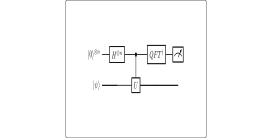
\includegraphics[width=0.7\textwidth]{../../images/qpe_circuit.svg}
\end{center}

\subsection{Mathematical Derivation}

QPE estimates eigenvalue $e^{2\pi i\theta}$ of unitary operator $U$:
\begin{equation}
U|\psi\rangle = e^{2\pi i\theta}|\psi\rangle
\end{equation}

QPE outputs $n$-bit approximation of $\theta$:
\begin{equation}
|0\rangle^{\otimes n}|\psi\rangle \xrightarrow{QPE} |\tilde{\theta}\rangle|\psi\rangle
\end{equation}

Where $\tilde{\theta} \approx \theta$, with precision $n$ bits.

\subsection{Geometric Interpretation}

QPE encodes phase information into control qubits on the Bloch sphere. Through inverse QFT, phase information is converted to measurable computational basis states.

\section{Code Walkthrough}

\begin{verbatim}
from quonic import qgate, qshow
from quonic.gates import H, X

# Prepare eigenstate |1>
qgate(X, 1)

# Create superposition
qgate(H, 0)

# Apply controlled-U
qgate(CU, 0, 1)

# Measure
qshow()
\end{verbatim}

\section{Advanced Usage}

\subsection{Scenario 1: Multi-bit QPE}

\begin{verbatim}
# Multi-bit QPE for higher precision
n = 3  # 3 control qubits
qgate(X, n)  # Prepare eigenstate
for i in range(n):
    qgate(H, i)
    qgate(CU, i, n)
qshow()
\end{verbatim}

\subsection{Scenario 2: QPE for Molecular Simulation}

\begin{verbatim}
# QPE for molecular simulation
# Estimate ground state energy
qgate(X, 3)  # Prepare molecular state
qgate(H, 0)
qgate(H, 1)
qgate(H, 2)
qgate(CU, 0, 3)
qgate(CU, 1, 3)
qgate(CU, 2, 3)
qshow()
\end{verbatim}

\section{Use Cases}

\subsection{Shor's Algorithm}

QPE is the core of Shor's algorithm, used to find periods.

\subsection{Quantum Chemistry}

QPE is used to estimate ground state energies of molecules.

\subsection{Quantum Machine Learning}

QPE is used in quantum kernel methods for eigenvalue estimation.

\section{FAQ}

\subsection{What is the precision of QPE?}

Precision is determined by the number of control qubits $n$. More qubits = higher precision.

\subsection{How many qubits does QPE need?}

QPE needs $n$ control qubits + 1 target qubit.

\subsection{What is the output of QPE?}

QPE output is a binary approximation of phase $\theta$.

\section{Learning Path}

\subsection{Prerequisites}
\begin{itemize}
  \item Quantum Fourier Transform (QFT)
  \item Controlled gates
  \item Quantum measurement
\end{itemize}

\subsection{Next Steps}
\begin{itemize}
  \item Shor's Algorithm
  \item Quantum Chemistry Simulation
  \item Quantum Machine Learning
\end{itemize}

\section{Complete Examples}

\subsection{Example 1: Basic QPE}

\begin{verbatim}
from quonic import qgate, qshow
from quonic.gates import H, X

qgate(X, 1)
qgate(H, 0)
qgate(CU, 0, 1)
qshow()
\end{verbatim}

\section{Download}

\begin{itemize}
  \item [qpe.py](https://github.com/ChrisLee0721/QuoNic/blob/main/examples/qpe/qpe.py)
\end{itemize}

\end{document}
